\section{Typy ramek HDLC}
	\subsection{Ramka XID}
	Jej nazwa pochodzi z języka angielskiego ,,exchange identification''. 
	Służy do przekazania urządzeniu podrzędnemu wiedzy na temat możliwości oraz charakterystyki komunikacji na warstwie łącza danych.
	
	Odpowiadając na tego typu wiadomości, urządzenie podrzędne najczęściej zwraca tę samą wartość w przypadku zgodności, 
	bądź najwyższą wspieraną, jeśli żądana jest zbyt duża. Szereg wysłanych i odebranych wiadomości XID nazywamy XID negocjacją.
	Tej ramki użyto również podczas ustalania prędkości komunikacji, co jest częścią procedury zestawienia warstwy fizycznej.
	Bajt kontrolny dla wiadomości przesyłanej ma zawsze wartość 0xBF. \newline
	Bajty budujące ramkę:
	\begin{itemize}
		\item Adresu;
		\item Kontrolny;
		\item Identyfikujący format;
		\item Identyfikujący grupę;
		\item Długości grupy;
		\item Parametrów HDLC:
		\begin{itemize}
			\item Identyfikujący parameter;
			\item Długości parameteru;
			\item Wartości parametru;
		\end{itemize}
	\end{itemize} 
	Wspomniano o parametrach HDLC, gdyż wiadomość negocjująca ich wartości może zawierać zarówno jeden jak i więcej parametrów.

	\begin{figure}[h!]
         \centering
         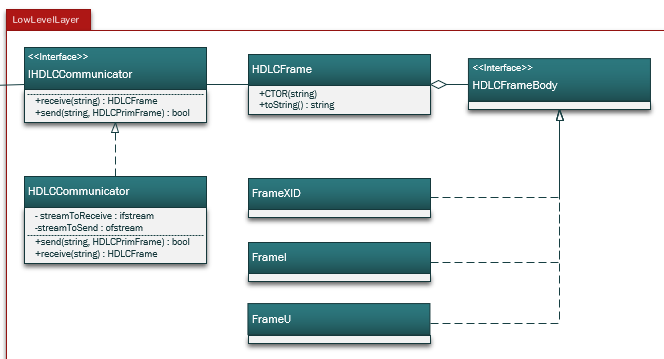
\includegraphics[scale=0.75]{Obrazki/DiagramyKlas/LowLevel.png}
         \caption{Diagram klas przedstawiający relację pomiędzy abstrakcyjną oraz konkretną klasą poszczególnej ramki.
             \newline(Opracowanie własne)}
    \end{figure}